
\subsection{Physics-Based Seismic Hazard Analysis}

Last, we present an application to seismic hazard analysis. Probabilistic seismic hazard analysis (PSHA) provides a technique to quantify seismic hazard while taking into account uncertainties in the models used to estimate ground motion levels. To help advance hazard analysis in southern California, SCEC has developed the CyberShake project, a physics-based framework to perform PSHA using 3D deterministic wave propagation simulations \citep{Graves_2011_PAG}.  CyberShake performs PSHA by simulating a tensor-valued wavefield of strain Green tensors, and uses seismic reciprocity to calculate synthetic seismograms for over 400,000 events per site of interest \citep{Zhao_2006_BSSA}. These seismograms are processed to obtain intensity measures, which are then combined with probabilities from an earthquake rupture forecast to produce a PSHA hazard curve. Hazard curves for hundreds of sites are combined into hazard maps, representing the seismic hazard across a region.

As in previous cases, one of the key inputs to CyberShake is the velocity model, which serves as the underlying material structure used to compute the strain Green tensors used in the hazard map construction. Initially, CyberShake was developed using custom wrappers for the CVM-S and CVM-H velocity models. This added complexity to the CyberShake code base, since specialized interfaces were required for each velocity model.

To simplify velocity mesh creation via a single interface, CyberShake transitioned to using UCVM upon its release. As a result, two large CyberShake studies were completed in 2013 \citep{Callaghan_2013_Proc} and 2014.  Each produced 4 hazard maps of the Los Angeles area, requiring the generation of 1,144 velocity meshes from UCVM, each with 1.2 billion mesh points. More important, CyberShake has been able to calculate hazard maps for 5 different velocity models in the Los Angeles area, all while using UCVM utilities. This has enabled detailed analysis of the impact of velocity models on seismic hazard. Through techniques such as averaging-based factorization (ABF), we have been able to quantify velocity model-dependent phenomena such as basin and directivity-basin coupling effects \citep{Wang_2014_BSSA}. A comparison of CyberShake hazard maps calculated with CVM-S4.26 and CVM-H is shown in Figure \ref{fig:cybershake} as representative of the analysis facilitated by UCVM.


\begin{figure}[ht!]
    \centering
    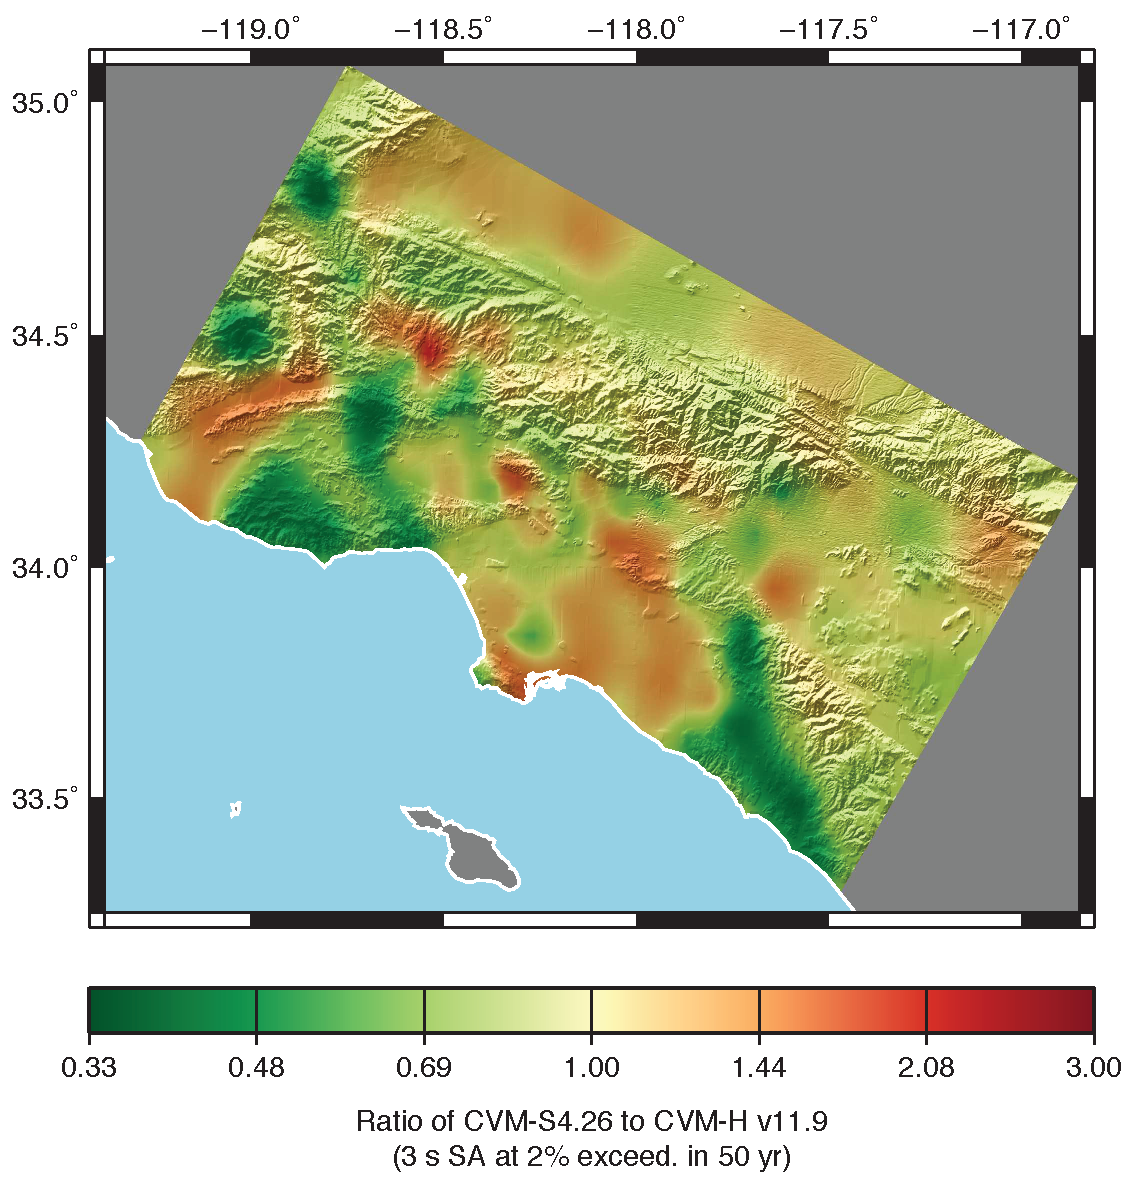
\includegraphics
        [width=0.9\columnwidth]
        {figures/pdf/cybershake}
    \caption{Ratio between two CyberShake seismic hazard maps obtained using two different velocity models, CVM-S4.26 and CVM-H. The underlying hazard maps correspond to a 3-seconds spectral acceleration with a 2\% chance of exceedance in 50 years. The discrete regular grids used as input for these computations were built using UCVM meshing utilities.}
    \label{fig:cybershake}
\end{figure}



